%; whizzy section -pdf xpdf -latex ./whizzypdfptex.sh
% latex beamer presentation.
% platex, latex-beamer でコンパイルすることを想定。 

%     Tokyo Debian Meeting resources
%     Copyright (C) 2007 Junichi Uekawa
%     Copyright (C) 2008 Nobuhiro Iwamatsu

%     This program is free software; you can redistribute it and/or modify
%     it under the terms of the GNU General Public License as published by
%     the Free Software Foundation; either version 2 of the License, or
%     (at your option) any later version.

%     This program is distributed in the hope that it will be useful,
%     but WITHOUT ANY WARRANTY; without even the implied warranty of
%     MERCHANTABILITY or FITNESS FOR A PARTICULAR PURPOSE.  See the
%     GNU General Public License for more details.

%     You should have received a copy of the GNU General Public License
%     along with this program; if not, write to the Free Software
%     Foundation, Inc., 51 Franklin St, Fifth Floor, Boston, MA  02110-1301 USA

\documentclass[cjk,dvipdfmx,12pt]{beamer}
\usetheme{Tokyo}
\usepackage{ulem}
\usepackage{tabularx}

\usepackage{fancybox}
\usepackage{fancyvrb}   
\usepackage{float}

\usepackage{txfonts}
\mathversion{bold}
\renewcommand{\familydefault}{\sfdefault}
\renewcommand{\kanjifamilydefault}{\gtdefault}
\setbeamerfont{title}{size=\large,series=\bfseries}
\setbeamerfont{frametitle}{size=\large,series=\bfseries}
\setbeamertemplate{frametitle}[default][center]
\usefonttheme{professionalfonts}

% commandline環境を定義。画面入出力についてはcommandline環境
% で表記する
\newenvironment{commandline}%
{\VerbatimEnvironment
  \begin{Sbox}\begin{minipage}{1.0\hsize}\begin{fontsize}{12}{12} \begin{BVerbatim}}%
{\end{BVerbatim}\end{fontsize}\end{minipage}\end{Sbox}
  \setlength{\fboxsep}{8pt}
% start on a new paragraph

\vspace{6pt}% skip before
\fcolorbox{dancerdarkblue}{dancerlightblue}{\TheSbox}

\vspace{6pt}% skip after
}
%end of commandline

\newenvironment{commandlinesmall}%
{\VerbatimEnvironment
  \begin{Sbox}\begin{minipage}{1.0\hsize}\begin{fontsize}{9}{9} \begin{BVerbatim}}%
{\end{BVerbatim}\end{fontsize}\end{minipage}\end{Sbox}
  \setlength{\fboxsep}{8pt}
% start on a new paragraph

\vspace{6pt}% skip before
\fcolorbox{dancerdarkblue}{dancerlightblue}{\TheSbox}

\vspace{6pt}% skip after
}
%end of commandlinesmall

\definecolor{dancerdarkblue}{rgb}{0,0.08,0.45}
\definecolor{dancernormalblue}{rgb}{0.8,0.9,0.95}
\definecolor{dancerlightblue}{rgb}{0.8,0.95,1}


%  preview (shell-command (concat "evince " (replace-regexp-in-string "tex$" "pdf"(buffer-file-name)) "&"))
%  presentation (shell-command (concat "xpdf -fullscreen " (replace-regexp-in-string "tex$" "pdf"(buffer-file-name)) "&"))

%http://www.naney.org/diki/dk/hyperref.html
%日本語EUC系環境の時
\AtBeginDvi{\special{pdf:tounicode EUC-UCS2}}
%シフトJIS系環境の時
%\AtBeginDvi{\special{pdf:tounicode 90ms-RKSJ-UCS2}}

\title{東京エリア Debian 勉強会}
\subtitle{Debian Package ハンズオン}
\author{岩松 信洋 iwamatsu@debian.or.jp\\IRC nick: iwamatsu}
\date{2008年03月01日}
\logo{
\includegraphics[width=8cm]{image200607/openlogo-light.eps}}


% 間のタイトルページ用
\newcommand{\emtext}[1]{
\begin{frame}{}
 
\begin{minipage}{0.55\hsize}
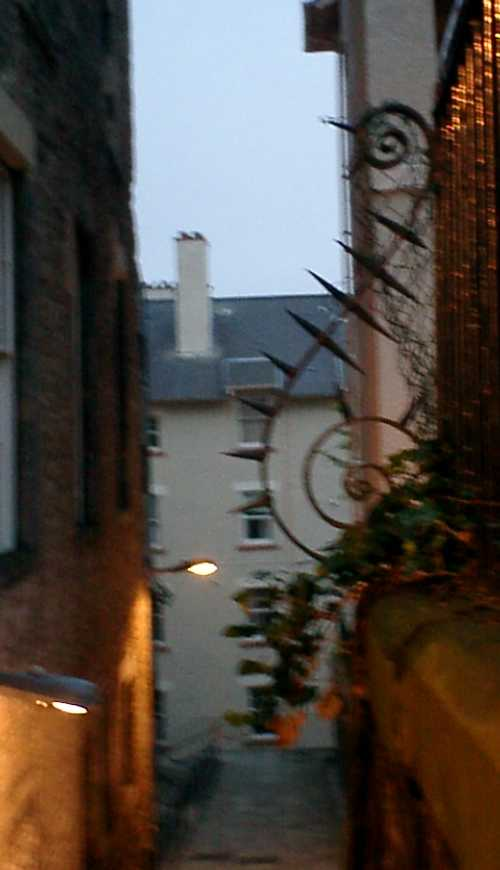
\includegraphics[width=1\hsize]{image200707/gurutitle.jpg}
\end{minipage}
\begin{minipage}{0.39\hsize}
 {\Huge #1
 }
\end{minipage}
\end{frame}
}

\begin{document}
\frame{\titlepage{}}

\section{Intro}

\emtext{Agenda}

\section{}
\begin{frame}
 \frametitle{Agenda}
  \begin{itemize}
  \item 今回の目的発表
  \item Debian Package を作成する前の準備
  \item 今回の生贄
  \item プログラムが動作を確認する
  \item Debian Package の雛形を作る
  \item debian/control ファイルの編集
  \item debian/changelog ファイルの編集
  \item debian/copyright ファイルの編集
  \item debian/rules ファイルを編集する
  \item Debian Package の作成
  \item Debian Package のテスト
  \item 本日のまとめ
  \item 終わりに
  \item 質疑応答
 \end{itemize}
\end{frame}

\section{今回の目的}
\emtext{今回の目的}

\begin{frame}
\alert{{\LARGE シングルバイナリの Debian Package が作成できるようになること。}}
\end{frame}

\section{Debian Package を作成する前の準備}
\emtext{Debian Package を作成する前の準備}

\section{Debian Package 作成環境}
\begin{frame}
以下の環境変数を設定しておくと便利。

\begin{itemize}
  \item DEBFULLNAME の設定

    Debian Package のメンテナ名
  \item DEBEMAIL の設定

    Debian Package  メンテナンス用のメールアドレス
\end{itemize}
\end{frame}

\begin{frame}[containsverbatim]

\begin{commandline}
$ cat ~/.bashrc
--略--
export DEBFULLNAME="Nobuhiro Iwamatsu"
export DEBEMAIL=iwamatsu@nigauri.org
--略--
$ source ~/.bashrc
\end{commandline}
\end{frame}

\begin{frame}{必要なパッケージ}
最低限必要な必要なパッケージは以下の通り。
\begin{itemize}
 \item devscripts
 \item debhelper
 \item lintian/linda
 \item gcc 
 \item binutils 
 \item libc6-dev
 \item dh-make
\end{itemize}

あると便利なパッケージ
\begin{itemize}
\item apt-file
\item pbuilder
\end{itemize}
\end{frame}

\section{今回の生贄}
\emtext{今回の生贄}

\begin{frame}[containsverbatim]
{\LARGE sl}
\begin{commandline}


      ====        ________                ___________
  _D _|  |_______/        \__I_I_____===__|_________|
   |(_)---  |   H\________/ |   |        =|___ ___|      _________________ 
   /     |  |   H  |  |     |   |         ||_| |_||     _|                \_____A
  |      |  |   H  |__--------------------| [___] |   =|                        |
  | ________|___H__/__|_____/[][]~\_______|       |   -|                        |
  |/ |   |-----------I_____I [][] []  D   |=======|____|________________________|_
__/ =| o |=-~~\  /~~\  /~~\  /~~\ ____Y___________|__|__________________________|_
 |/-=|___||    ||    ||    ||    |_____/~\___/          |_D__D__D_|  |_D__D__D_|
  \_/      \__/  \__/  \__/  \__/      \_/               \_/   \_/    \_/   \_/

\end{commandline}
\end{frame}

\section{プログラムが動作を確認する}
\emtext{プログラムが動作を確認する}

\begin{frame}[containsverbatim]
まず、プログラムが動作するか確認しましょう。
\begin{commandline}
$ tar -xf sl.tar
$ cd sl
$ make
\end{commandline}
\end{frame}

\begin{frame}[containsverbatim]
curses.h がないため、コンパイルに失敗しました。
\begin{commandline}
$ tar -xf sl.tar
$ cd sl
$ make
 make
cc -O -o sl sl.c -lcurses -ltermcap
sl.c:30:20: error: curses.h: No such file or directory
sl.c: In function 'my_mvaddstr':
sl.c:42: error: 'ERR' undeclared (first use in this function)
sl.c:42: error: (Each undeclared identifier is reported only once
........ 
\end{commandline}
\end{frame}

\begin{frame}[containsverbatim]
curses.h を持った Debian Package が必要です。
どのファイルがどのパッケージじよってインストールされるのか、調べるには
\alert{apt-file}を使うと便利です。
\begin{commandline}
# sudo apt-file update
$ apt-file search /usr/include/curses.h
libncurses5-dev: usr/include/curses.h
\end{commandline}
\end{frame}

\begin{frame}[containsverbatim]
\alert{libncueses5-dev} パッケージをインストールして再度コンパイルしましょう。
\begin{commandline}
# apt-get update
# apt-get install libncurses5-dev
$ make
 make
cc -O -o sl sl.c -lcurses -ltermcap
.......
\end{commandline}
\end{frame}

\begin{frame}[containsverbatim]
コンパイルが通ったので、動作テストをしましょう。
\begin{commandline}
% ./sl
\end{commandline}
\end{frame}

\section{Debian Package の雛形を作る}
\emtext{Debian Package の雛形を作る}

\begin{frame}[containsverbatim]
ディレクトリにバージョンがない場合はバージョンが付いたディレクトリ名に変更します。
Debian Package の雛形を作成するには、dh\_make コマンドを使います。

%Debian Package はパッケージのバージョンを要求します。ディレクトリにバージョンが
%ない場合はバージョンが付いたディレクトリ名に変更します。
\begin{commandline}
$ tar -xf sl.tar
$ mv sl sl-0.0.0
$ cd sl-0.0.0
$ dh_make 
\end{commandline}
\end{frame}

\begin{frame}[containsverbatim]
\begin{commandline}
iwamatsu@chimagu:~/sl-0.0.0$ dh_make

Type of package: single binary, multiple binary, 
library, kernel module or cdbs?
 [s/m/l/k/b] 
\end{commandline}
\end{frame}

\begin{frame}
\begin{itemize}
  \item s: 一つの実行バイナリを提供するパッケージ
  \item m: 2つ以上の実行バイナリを提供するパッケージ
  \item l: ライブラリ用パッケージ
  \item k: カーネルモジュール用パッケージ
  \item b: cdbs を使ったパッケージ
\end{itemize}
\end{frame}

\begin{frame}[containsverbatim]
\begin{commandline}
$ dh_make

Type of package: single binary, multiple binary, 
library, kernel module or cdbs?
 [s/m/l/k/b] s
Maintainer name : Nobuhiro Iwamatsu
Email-Address   : iwamatsu@nigauri.org 
Date            : Thu, 21 Feb 2008 15:46:57 +0900
Package Name    : sl
Version         : 0.0.0
License         : blank
Type of Package : Single
Hit <enter> to confirm:
\end{commandline}
\end{frame}

\begin{frame}[containsverbatim]
\begin{commandline}
$ dh_make

Type of package: single binary, multiple binary, 
library, kernel module or cdbs?
 [s/m/l/k/b] s
Maintainer name : Nobuhiro Iwamatsu
Email-Address   : iwamatsu@nigauri.org 
Date            : Thu, 21 Feb 2008 15:46:57 +0900
Package Name    : sl
Version         : 0.0.0
License         : blank
Type of Package : Single
Hit <enter> to confirm:
 
Could not find sl_0.0.0.orig.tar.gz
Either specify an alternate file to use with -f,
or add --createorig to create one.
\end{commandline}
\end{frame}

\begin{frame}[containsverbatim]
xxx.orig.tar.gz がないと、エラーになります。\\
--createorig オプションを加えて dh\_makeを実行しましょう。

\begin{commandline}
$ dh_make --createorig
\end{commandline} 
\end{frame}

\section{}

\begin{frame}[containsverbatim]

dh\_make 実行後、debian ディレクトリが作成されます。
\begin{commandline}
$ ls ./debian/
README.Debian  control    dirs  emacsen-remove.ex   
init.d.lsb.ex  manpage.xml.ex   mogeri.doc-base.EX  
preinst.ex     watch.ex  changelog  copyright  
docs           emacsen-startup.ex manpage.1.ex     
menu.ex        postinst.ex      prerm.ex
compat         cron.d.ex        emacsen-install.ex  
init.d.ex      manpage.sgml.ex  sl-default.ex  
postrm.ex      rules
\end{commandline}
\end{frame}

\begin{frame}[containsverbatim]
*.ex / *.EX はサンプルなので削除します。
\begin{commandline}
$ rm -rf ./debian/*.ex
$ rm -rf ./debian/*.EX
\end{commandline}
\end{frame}

\begin{frame}[containsverbatim]

最低限必要な debian ディレクトリ以下にあるファイルは以下の通りです。。

\begin{itemize}
  \item README.Debian -- Package のREADME
  \item control       -- Package の説明、ビルドに必要な情報など
  \item dirs          -- Package で利用するディレクトリを記述
  \item changelog     -- Package の変更履歴
  \item copyright     -- Package のコピーライト
  \item docs          -- ドキュメントファイル一覧
  \item rules         -- Package 作成用のスクリプト(Makefile)
  \item compat        -- debhelper のバージョン
\end{itemize}
\end{frame}

\section{debian/control ファイルの編集}
\emtext{debian/control ファイルの編集}

\begin{frame}[containsverbatim]
\begin{commandline}
Source: sl
Section: game
Priority: extra
Maintainer: Nobuhiro Iwamatsu <iwamatsu@nigauri.org>
Build-Depends: debhelper (>= 5),libncurses5-dev
Standards-Version: 3.7.2

Package: sl
Architecture: any
Depends: ${shlibs:Depends}, ${misc:Depends}
Description: Key type correction software
 Key type correction software for 'ls' command.
\end{commandline}
\end{frame}

\section{debian/changelog ファイルの編集}
\emtext{debian/changelog ファイルの編集}

\begin{frame}[containsverbatim]

次に Debian の Changelog を編集しましょう。
編集するには、dch コマンドを使います。

\begin{commandline}
$ dch 
sl (0.0.0-1) unstable; urgency=low

  * Initial release

 -- Nobuhiro Iwamatsu <iwamatsu@nigauri.org> \
     Sun, 24 Feb 2008 01:01:53 +0900

\end{commandline}
\end{frame}

\section{debian/copyright ファイルの編集}
\emtext{debian/copyright ファイルの編集}

\begin{frame}[containsverbatim]
\begin{commandlinesmall}
This package was debianized by \ 
Nobuhiro Iwamatsu <iwamatsu@nigauri.org> on
Thu, 21 Feb 2008 16:13:47 +0900.

It was downloaded from http://www.is.titech.ac.jp/~toyoda/

Upstream Author:
 Toyoda Masashi <toyoda@is.titech.ac.jp>

Copyright:

 Copyright 1993,1998 Toyoda Masashi (toyoda@is.titech.ac.jp)

License:
 Everyone is permitted to do anything on this program 
 including copying,
 modifying, and improving, unless you try to pretend that 
 you wrote it.
 i.e., the above copyright notice has to appear in all copies.
 THE AUTHOR DISCLAIMS ANY RESPONSIBILITY WITH REGARD TO 
 THIS SOFTWARE.

The Debian packaging is \
(C) 2008, Nobuhiro Iwamatsu <iwamatsu@nigauri.org> and
is licensed under the GPL, see `/usr/share/common-licenses/GPL'.

# Please also look if there are files or directories which have a
# different copyright/license attached and list them here.
\end{commandlinesmall}
\end{frame}

\begin{frame}
めんどくさいので、コピー。
\end{frame}

\begin{frame}
実際は、ソフトウェアの著作権を持っている人に連絡をとり、ライセンスを確認する必要があります。
\end{frame}

\section{debian/rules ファイルを編集する}
\emtext{debian/rules ファイルを編集する}
\begin{frame}[containsverbatim]
debian/rules は Debian Package を作成する Makefile です。
\begin{itemize}
 \item configure ターゲット
 \item build ターゲット
 \item clean ターゲット
 \item install ターゲット
\end{itemize}
\end{frame}

\begin{frame}[containsverbatim]
今回はシンプルなプログラムなので、変更する必要はありません。
\end{frame}

\section{とりあえず Package を作成する}
\emtext{とりあえず Package を作成する}
\begin{frame}[containsverbatim]

Debian Package を作る時は、\alert{debuild} コマンドを使います。
\begin{commandline}
$ debuild -us -uc
\end{commandline}
-us ソースパッケージにGPGサインをしない

-uc *.changes ファイルに GPG サインをしない

\end{frame}

\begin{frame}[containsverbatim]
\begin{commandline}
$ debuild -us -uc
 fakeroot debian/rules clean
dh_testdir
dh_testroot
rm -f build-stamp configure-stamp
# Add here commands to clean up after the \
build process.
/usr/bin/make clean
make[1]: ディレクトリ `/tmp/sl-0.0.0' に入ります
make[1]: *** ターゲット `clean' を make するルール \
がありません.  中止.
make[1]: ディレクトリ `/tmp/sl-0.0.0' から出ます
make: *** [clean] エラー 2
debuild: fatal error at line 1239:
fakeroot debian/rules clean failed
\end{commandline}
\end{frame}

\section{Makefile の修正}
\emtext{Makefile の修正}
\begin{frame}[containsverbatim]

図rules ファイルとMakefile の関係図
今のMakefile
\begin{commandline}
CC=cc
CFLAGS=-O

sl: sl.c sl.h
  $(CC) $(CFLAGS) -o sl sl.c -lcurses -ltermcap
# $(CC) $(CFLAGS) -o sl sl.c -lcurses
\end{commandline}
\end{frame}

\begin{frame}[containsverbatim]
修正後
\begin{commandline}
CC=cc
CFLAGS=-O
BINDIR?=/usr/games/ <--- インストール先を追加

\end{commandline}
\alert{BINDIR} : 実行バイナリがインストールされるディレクトリ
\end{frame}

\begin{frame}[containsverbatim]
修正後
\begin{commandline}

install:  <-- install ターゲットを追加
  install -d ${DESTDIR}${BINDIR}
  install -m 755 sl ${DESTDIR}${BINDIR}

clean:    <-- clean ターゲットを追加
  rm -rf sl

\end{commandline}
\alert{DESTDIR}: Debian Package のインストールされる TOP ディレクトリ
\end{frame}

\section{再度Debian Packageを作成}
\emtext{再度Debian Packageを作成}
\begin{frame}[containsverbatim]
\begin{commandline}
$ debuild -us -uc
......
dh_shlibdeps
dh_gencontrol
dpkg-gencontrol: warning: unknown substitution variable ${misc:Depends}
dh_md5sums
dh_builddeb
dpkg-deb: building package `sl' in `../sl_0.0.0-1_i386.deb'.
 dpkg-genchanges
dpkg-genchanges: including full source code in upload
dpkg-buildpackage (debuild emulation): full upload (original source is included)
Now running lintian...
W: sl: binary-without-manpage sl
Finished running lintian.
\end{commandline}
\end{frame}

\section{Debian Packageのテスト}
\emtext{Debian Package のテスト}

\section{}
\begin{frame}[containsverbatim]
\begin{itemize}
  \item pbuilder

   最低限のDebian systemから、パッケージを作成するためのツール。 

   \begin{commandline}
$ sudo /usr/sbin/pbuilder build sl_0.0.0-1.dsc 
   \end{commandline}
  \item piuparts 

   Debian Package の インストール/アンインストールのチェックをするためのツール。

\end{itemize}
\end{frame}

\section{まとめ}
\emtext{本日のまとめ}

\section{}
\begin{frame}
\begin{itemize}
  \item まずは、ソフトウェアが動作するか確認する
  \item dh\_make コマンド でパッケージの雛形を作成する
  \item debuild コマンド でパッケージ作成
  \item ライセンスやコピーライトの確認をすること
  \item lintian/linda で パッケージのチェック
  \item インストールして動作確認まで行う
  \item アンインストールの確認も忘れずに
\end{itemize}
\end{frame}

\section{情報源}
\emtext{情報源}
\begin{frame}
\begin{itemize}
  \item Debian Project / Debian JP Project Website

    \url{http://www.debian.org}

    \url{http://www.debian.or.jp}

  \item 東京エリアDebian勉強会

    \url{http://tokyodebian.alioth.debian.org}
  \item Debian Policy
    
    \url{http://www.debian.org/doc/debian-policy/}

  \item Debian 新メンテナガイド
    
    \url{http://www.debian.org/doc/manuals/maint-guide/index.ja.html}
\end{itemize}
\end{frame}

\section{終わりに}
\emtext{終わりに}

\section{}
\begin{frame}
今年のDebian勉強会では、毎月様々なDebian Pakcage の
作成方法をみなさんに伝授します。
\begin{itemize}
  \item データだけのDebianPackage作成方法
  \item VCSを使ったDebian Packageの作成方法
  \item ライブラリのDebian Package 作成方法
  \item などなど
\end{itemize}
\end{frame}


\section{質疑応答}
\emtext{質疑応答}

\end{document}

;;; Local Variables: ***
;;; outline-regexp: "\\([ 	]*\\\\\\(documentstyle\\|documentclass\\|emtext\\|section\\|begin{frame}\\)\\*?[ 	]*[[{]\\|[]+\\)" ***
;;; End: ***
